\documentclass[11pt,a4paper]{article}

%------------------------------------------------------------------------------
%	REQUIRED PACKAGES AND  CONFIGURATIONS
%------------------------------------------------------------------------------

% PACKAGES FOR TITLES
\usepackage{titlesec}
\usepackage{color}

% PACKAGES FOR LANGUAGE AND FONT
\usepackage[utf8]{inputenc}
\usepackage[italian]{babel}
\usepackage[T1]{fontenc} % Font encoding
\usepackage{kpfonts}
\tolerance=1
\emergencystretch=\maxdimen
\hyphenpenalty=10000
\hbadness=10000

% PACKAGES FOR IMAGES
\usepackage{graphicx}
\graphicspath{{Images/}} % Path for images' folder
\usepackage{eso-pic} % For the background picture on the title page
\usepackage{subfig} % Numbered and caption subfigures using \subfloat
\usepackage{caption} % Coloured captions
\usepackage{transparent}

% STANDARD MATH PACKAGES
\usepackage{amsmath}
\usepackage{amsthm}
\usepackage{bm}
\usepackage[overload]{empheq}  % For braced-style systems of equations

% PACKAGES FOR TABLES
\usepackage{tabularx}
\usepackage{longtable} % tables that can span several pages
\usepackage{colortbl}

% PACKAGES FOR ALGORITHMS (PSEUDO-CODE)
\usepackage{algorithm}
\usepackage{algorithmic}

% PACKAGES FOR REFERENCES & BIBLIOGRAPHY
\usepackage[colorlinks=true,linkcolor=black,anchorcolor=black,citecolor=black,filecolor=black,menucolor=black,runcolor=black,urlcolor=black]{hyperref} % Adds clickable links at references
\usepackage{cleveref}
\usepackage[square, numbers, sort&compress]{natbib} % Square brackets, citing references with numbers, citations sorted by appearance in the text and compressed
\bibliographystyle{plain} % You may use a different style adapted to your field

% PACKAGES FOR THE APPENDIX
\usepackage{appendix}

% PACKAGES FOR ITEMIZE & ENUMERATES 
\usepackage{enumitem}

% OTHER PACKAGES
\usepackage{amsthm,thmtools,xcolor} % Coloured "Theorem"
\usepackage{comment} % Comment part of code
\usepackage{fancyhdr} % Fancy headers and footers
\usepackage{lipsum} % Insert dummy text
\usepackage{tcolorbox} % Create coloured boxes (e.g. the one for the key-words)
\usepackage{stfloats} % Correct position of the tables
\usepackage{cuted}

%-------------------------------------------------------------------------
%	NEW COMMANDS DEFINED
%-------------------------------------------------------------------------

% EXAMPLES OF NEW COMMANDS -> here you see how to define new commands
\newcommand{\bea}{\begin{eqnarray}} % Shortcut for equation arrays
\newcommand{\eea}{\end{eqnarray}}
\newcommand{\e}[1]{\times 10^{#1}}  % Powers of 10 notation
\newcommand{\mathbbm}[1]{\text{\usefont{U}{bbm}{m}{n}#1}} % From mathbbm.sty
\newcommand{\pdev}[2]{\frac{\partial#1}{\partial#2}}
% NB: you can also override some existing commands with the keyword \renewcommand

%----------------------------------------------------------------------------
%	ADD YOUR PACKAGES (be careful of package interaction)
%----------------------------------------------------------------------------


%----------------------------------------------------------------------------
%	ADD YOUR DEFINITIONS AND COMMANDS (be careful of existing commands)
%----------------------------------------------------------------------------
\newcommand{\twofig}[6]{
\begin{figure}[H]
	\begin{minipage}{0.48\linewidth}
		\centering
		\includegraphics[width=\linewidth]{#1}
		\caption{#2}
		\label{fig:#3}
	\end{minipage}\hfill
	\begin{minipage}{0.48\linewidth}
		\centering
		\includegraphics[width=\linewidth]{#4}
		\caption{#5}
		\label{fig:#6}
	\end{minipage}
\end{figure}
}

\newcommand{\cfig}[4]{
\begin{figure}[H]
	\centering
	\includegraphics[width=#4\linewidth]{#1}
	\caption{#2}
	\label{fig:#3}
\end{figure}
}


% Do not change Configuration_files/config.tex file unless you really know what you are doing. 
% This file ends the configuration procedures (e.g. customizing commands, definition of new commands)
% Set the geometric layout of the document
\usepackage{geometry}
\geometry{
  top=3cm,
  left = 2.0cm,
  right = 2.0cm,
  bottom=2cm,
  headheight= 2.2cm,
  headsep= 0cm,
}
\raggedbottom 

% Create color bluePoli (-> manuale grafica coordinata:  https://www.polimi.it/fileadmin/user_upload/il_Politecnico/grafica-coordinata/2015_05_11_46xy_manuale_grafica_coordinata.pdf)
\definecolor{bluePoli}{cmyk}{0.4,0.1,0,0.4}

% Custom theorem environments
\declaretheoremstyle[
  headfont=\color{bluePoli}\normalfont\bfseries,
  bodyfont=\color{black}\normalfont\itshape,
]{colored}

\captionsetup[figure]{labelfont={color=bluePoli}} % Set colour of the captions
\captionsetup[table]{labelfont={color=bluePoli}} % Set colour of the captions
\captionsetup[algorithm]{labelfont={color=bluePoli}} % Set colour of the captions

\theoremstyle{colored}
\newtheorem{theorem}{Theorem}[section]
\newtheorem{proposition}{Proposition}[section]

% Enhances the features of the standard "table" and "tabular" environments.
\newcommand\T{\rule{0pt}{2.6ex}}
\newcommand\B{\rule[-1.2ex]{0pt}{0pt}}

% Algorithm description
\newcounter{algsubstate}
\renewcommand{\thealgsubstate}{\alph{algsubstate}}
\newenvironment{algsubstates}{
    \setcounter{algsubstate}{0}%
    \renewcommand{\STATE}{%
    \stepcounter{algsubstate}%
    \Statex {\small\thealgsubstate:}\space}
    }{}
    
% Custom theorem environment
\newcolumntype{L}[1]{>{\raggedright\let\newline\\\arraybackslash\hspace{0pt}}m{#1}}
\newcolumntype{C}[1]{>{\centering\let\newline\\\arraybackslash\hspace{0pt}}m{#1}}
\newcolumntype{R}[1]{>{\raggedleft\let\newline\\\arraybackslash\hspace{0pt}}m{#1}}

% Custom itemize environment
\setlist[itemize,1]{label=$\bullet$}
\setlist[itemize,2]{label=$\circ$}
\setlist[itemize,3]{label=$-$}
\setlist{nosep}

% Set separation of columns 
\setlength{\columnsep}{40pt}

% Create command for background pic
\newcommand\BackgroundPic{% Adding background picture
	\put(230,358){
		\parbox[b][\paperheight]{\paperwidth}{%
			\vfill
			\centering
			\transparent{0.4}
			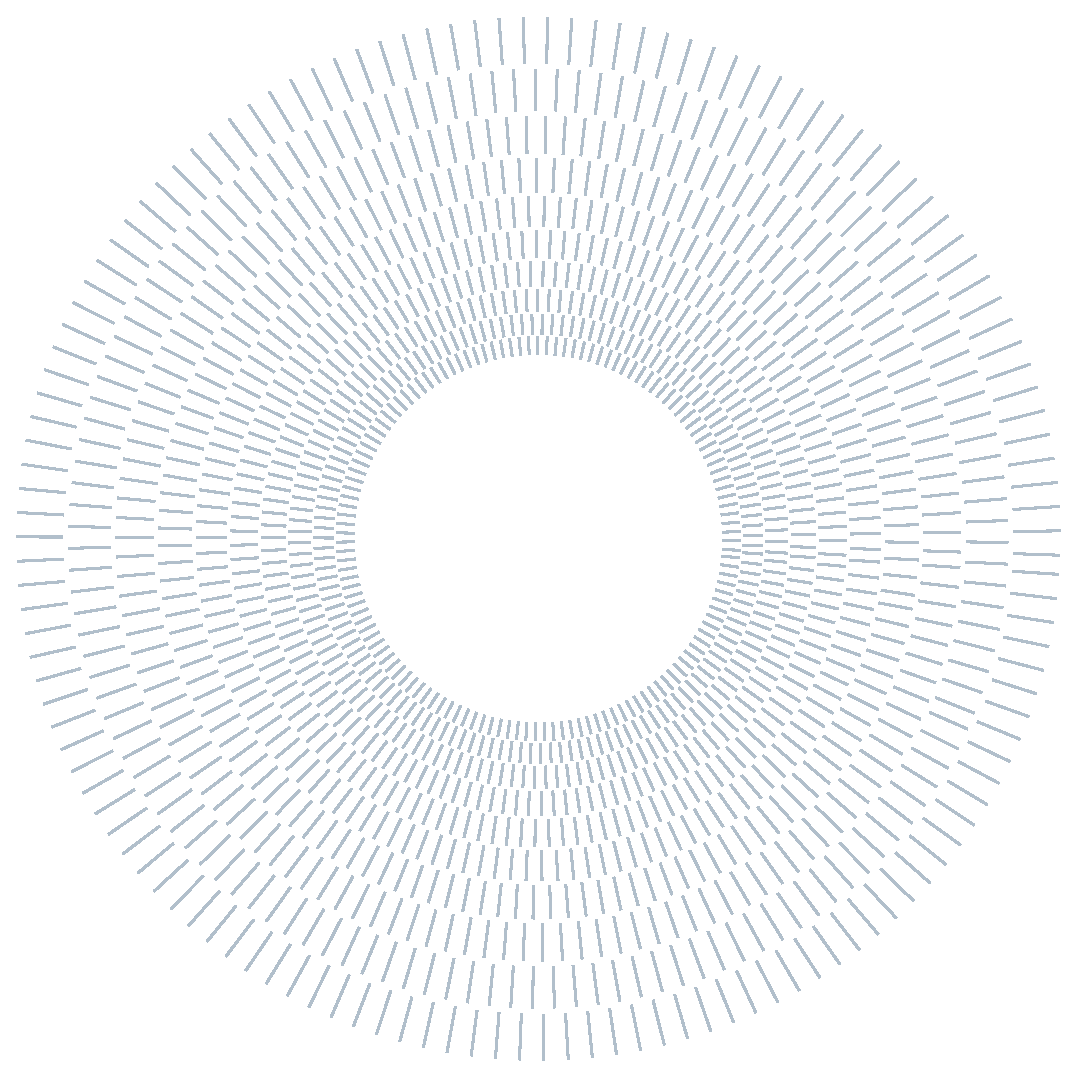
\includegraphics[width=0.5\paperwidth]{raggiera_polimi.eps}%
			\vfill
}}}

% Set indentation
\setlength\parindent{0pt}

% Custom title commands
\titleformat{\section}
{\color{bluePoli}\normalfont\Large\bfseries}
{\color{bluePoli}\thesection.}{1em}{}
\titlespacing*{\section}
{0pt}{2ex}{1ex}

\titleformat{\subsection}
{\color{bluePoli}\normalfont\large\bfseries}
{\color{bluePoli}\thesubsection.}{1em}{}
\titlespacing*{\subsection}
{0pt}{2ex}{1ex}

% Custom headers and footers
\pagestyle{fancy}
\fancyhf{}
      
\fancyfoot{}
\fancyfoot[C]{\thepage} % page
\renewcommand{\headrulewidth}{0mm} % headrule width
\renewcommand{\footrulewidth}{0mm} % footrule width

\makeatletter
\patchcmd{\headrule}{\hrule}{\color{black}\hrule}{}{} % headrule
\patchcmd{\footrule}{\hrule}{\color{black}\hrule}{}{} % footrule
\makeatother

% -> Create the header
\chead[C]{
\centering
\begin{tcolorbox}[arc=0pt, boxrule=0pt, colback=bluePoli!60, width=\textwidth, colupper=white]
    \textbf{Prova Finale di Propulsione Aerospaziale} \hfill \textbf{\author}  
\end{tcolorbox}
}

%----------------------------------------------------------------------------

% Insert here the info that will be displayed into your Title page 
% -> title of your work
\renewcommand{\title}{Prova Finale di Propulsione Aerospaziale}

% -> author name and surname
\newcommand{\authors}{Alex Cristian Turcu, Giorgia Pallara, Silvia Pala, Reshal Antonino Fernando Warnakulasuriya,\\\hspace*{10mm} Daniele Paternoster}

% -> MSc course
\newcommand{\course}{Aerospace Engineering - Ingegneria Aerospaziale}

% -> advisor name and surname
\newcommand{\professor}{Christian Paravan}

% IF AND ONLY IF you need to modify the co-supervisors you also have to modify the file Configuration_files/title_page.tex (ONLY where it is marked)
%\newcommand{\firstcoadvisor}{Name Surname} % insert if any otherwise comment
%\newcommand{\secondcoadvisor}{Name Surname} % insert if any otherwise comment

% -> academic year
\newcommand{\YEAR}{2022-2023}

\begin{document}

%-----------------------------------------------------------------------------
% TITLE PAGE
%-----------------------------------------------------------------------------

% Do not change Configuration_files/TitlePage.tex (Modify it IF AND ONLY IF you need to add or delete the Co-advisors)
% This file creates the Title Page of the document
% DO NOT REMOVE SPACES BETWEEN LINES!

\twocolumn[{\begin{@twocolumnfalse}

\AddToShipoutPicture*{\BackgroundPic}

\hspace{-0.6cm}
\includegraphics[width=0.6\textwidth]{logo_polimi_ing_indinf.eps}

\vspace{-0.2cm}
\Large{\textbf{\color{bluePoli}{\title}}}\\
\hspace*{\fill}

\vspace{-0.2cm}
\fontsize{0.3cm}{0.5cm}\selectfont \bfseries \textsc{\color{bluePoli} Laurea Magistrale in \course}\\
\hspace*{\fill}

\vspace{-0.2cm}
\fontsize{0.3cm}{0.5cm} \selectfont \bfseries Autori: \textsc{\textbf{\authors}}\\
\hspace*{\fill}

\vspace{-0.4cm}
\fontsize{0.3cm}{0.5cm}\selectfont \bfseries Professore: \textsc{\textbf{\professor}}\\
\hspace*{\fill}

% if only ONE co-advisor is present:
%\vspace{-0.4cm}
%\fontsize{0.3cm}{0.5cm}\selectfont \bfseries Co-advisor: %\textsc{\textbf{\firstcoadvisor}}\\
% if more than one co-advisors are present:
%\vspace{-0.4cm}
%\fontsize{0.3cm}{0.5cm}\selectfont \bfseries Co-advisors: \textsc{\textbf{\firstcoadvisor}}\textsc{\textbf{\secondcoadvisor}}\\

\vspace{-0.4cm}
\fontsize{0.3cm}{0.5cm}\selectfont \bfseries Anno accademico: \textsc{\textbf{\YEAR}}

\small \normalfont

\vspace{11pt}

\centerline{\rule{1.0\textwidth}{0.4pt}}

\vspace{15pt}
\end{@twocolumnfalse}}]

\thispagestyle{plain} % In order to not show the header in the first page

\vspace{15mm}
\begin{abstract}
	\vspace*{5mm}
La presente relazione di prova finale intende dare una descrizione dell'endoreattore F-1 prodotto da Rocketdyne. Cinque di questi motori vennero installati sul primo stadio S-IC del vettore Saturn V che portò il primo uomo sulla luna. L'obiettivo di questo stadio era quello di portare il razzo ad una quota di 61 km, fornendo un $\Delta v \simeq $ 2300 m/s.\\
Di seguito verranno analizzati i principali sistemi per un singolo motore, partendo dal sistema di alimentazione, passando per il sistema di generazione della potenza ed arrivando infine al sistema di espansione gasdinamico e al suo raffreddamento. Si provvederà inoltre a dare una descrizione quali/quantitativa delle scelte progettuali applicate ai tempi. Infine, verrà studiata una alternativa ai propellenti utilizzati, rimarcando le conseguenze sull'intero sistema propulsivo che tale variazione implica.
\end{abstract}

\clearpage

%-----------------------------------------------------------------------------


\section{Nomenclatura}

\label{sec:nomenclatura}


%-----------------------------------------------------------------------------


\section{Analisi della missione}

\label{sec:analisi missione}

La missione prevede una durata totale di funzionamento dello stadio di 161 s, durante il quale l’obiettivo principale è quello di portare il vettore di lancio ad una altitudine approssimativa di 61 km e ad una velocità di circa 2388 m/s. La sequenza di accensione prevede l’avvio del motore centrale per primo, seguito in sequenza dalle due coppie di motori simmetrici, questi accesi con un ritardo di 300 ms allo scopo di ridurre al minimo le vibrazioni sulla struttura principale; il computer di bordo attende quindi il raggiungimento del valore di spinta massimo per inviare il comando di sgancio del razzo dalla rampa di lancio. Il vettore, una volta sganciato, non può più essere fermato. Ad un’altitudine fissata di 1300 metri, il Saturn V comincia una manovra di rollio attorno al suo asse al fine di raggiungere la traiettoria corretta per il prosieguo della missione. La totalità delle informazioni riguardanti le istruzioni per l’assetto e i venti dominanti nel periodo di lancio sono pre-registrate nel programma di lancio. È inoltre necessario lo spegnimento del motore centrale a t = 135 s, prefissato da programma, per non superare i limiti strutturali di carico massimo sopportabile. La spinta, infatti, non è un fattore controllabile nei motori F-1 e, per ovviare a questo problema, si provvede quindi ad interrompere direttamente il flusso di propellente al motore.

Di seguito sono riportate le formule e i risultati di una simulazione della missione del primo stadio del Saturn V, il cui scopo è di analizzare le variazioni dei vari parametri di interesse del razzo durante tutto il tempo di volo. Tale simulazione è stata realizzata con l'ausilio del software MATLAB, con il quale è stato risolto il sistema di equazioni differenziali descritto più avanti. L'algoritmo numerico risolutivo scelto è il metodo di Eulero in avanti.

Per la simulazione del lancio è stato sviluppato un modello con determinate ipotesi semplificative al fine di descrivere l’intera dinamica del razzo:

\begin{itemize}[wide,itemsep=3pt,topsep=3pt]
\item
è stato utilizzato un modello di Terra piatta ed irrotazionale, al fine di adottare un sistema di riferimento inerziale, trascurando dunque effetti di variazione di traiettoria dovuti allo spostamento terrestre e variazioni di quota dovute al cambiamento di latitudine durante il volo;
\item
i valori di pressione e temperatura ambientale al variare della quota sono stati ottenuti mediante l'uso del Modello di Atmosfera Standard, ponendo una temperatura di riferimento al suolo di 25°C;
\item
il valore di portata massica del propellente ai motori è assunto costante durante tutto il funzionamento dello stadio, con una variazione del suo valore soltanto a seguito dello spegnimento del motore centrale al tempo prefissato;
\item
per ricavare le forze di resistenza aerodinamica è stata usata una curva empirica del coefficiente di drag al variare del numero di Mach.
% qua mettiamo la reference al sito da cui abbiamo trovato i dati del Cd
\end{itemize}

Il modello matematico realizzato per la descrizione del vettore di lancio consta dunque delle seguenti equazioni:

\begin{empheq}{gather*}
	h = \frac{dv_{v}}{dt}									\qquad
	v_{v} = \frac{da_{v}}{dt}								\qquad
	v_{h} = \frac{da_{h}}{dt}								\qquad
	v_{tot} = \sqrt{v_{v}^2 + v_{h}^2}						\\
	\phi = \arctan \frac{v_{h}}{v_{v}}						\qquad
	a_{v} = -g + \frac{T \cos \theta - D \cos \phi}{m}		\qquad
	a_{h} = \frac{T \sin \theta - D \sin \phi}{m}				\\
	g = \frac{\mu}{\left( R_T + h \right) ^2}					\qquad
	m = m_i - \dot{m} t										\qquad
	T = T_{vac} - A_e p_e									\qquad
	D = \frac{1}{2} \, \rho \, v_{tot}^2 \, S \, C_D
\end{empheq}
\vspace*{5mm}

Seppur il modello risulti semplificato rispetto alla complessa realtà fisica di funzionamento, si ottengono andamenti delle principali grandezze fisiche di interesse perfettamente in linea con gli andamenti tabellati forniti nei manuali di volo del vettore di lancio.	% qua mettiamo la reference ai dati reali
I requisiti fondamentali, ovvero il raggiungimento della quota prefissata e della velocità finale prima dello sgancio dello stadio S-IC, risultano soddisfatti e sufficientemente precisi, con un valore ottenuto di 59557 m (errore percentuale di 000\% rispetto al reale) e 2353 m/s (errore percentuale di 000\%).	% sostituire i dati trovati

Di seguito sono riportati i grafici di alcune grandezze in funzione del tempo di volo:

%\figura{01_quota_t}{Quota in funzione del tempo}{quota_t}
%\figura{02_velocita_t}{Velocità in funzione del tempo}{velocita_t}
%\figura{03_accelerazione_t}{Accelerazione in funzione del tempo}{accelerazione_t}
%\figura{04_spinta_t}{Spinta in funzione del tempo}{spinta_t}
%\figura{05_drag_t}{Drag in funzione del tempo}{drag_t}
%\figura{06_massa_t}{Massa totale in funzione del tempo}{massa_t}
%\figura{07_traiettoria}{Traiettoria del vettore}{traiettoria}

\twofig{01_quota_t}{Quota in funzione del tempo}{quota_t}{02_velocita_t}{Velocità in funzione del tempo}{velocita_t}

\cfig{04_spinta_t}{Spinta in funzione del tempo}{spinta_t}{0.48}

Le evidenze sperimentali ci permettono quindi di assumere il modello implementato come effettivamente rappresentativo del lancio del Saturn V avvenuto nella realtà.


%-----------------------------------------------------------------------------


\section{Analisi dei propellenti}

\label{sec:analisi propellenti}


%-----------------------------------------------------------------------------


\section{Dimensionamento dei tank}

\label{sec:dimensionamento tank}


%-----------------------------------------------------------------------------


\section{Schema termodinamico}

\label{sec:schema termodinamico}


%-----------------------------------------------------------------------------


\section{Gas generator}

\label{sec:gas generator}

Le difficoltà progettuali incontrate per il design del GG furono molte: vennero sviluppate molte geometrie diverse negli anni precedenti. Per ovviare a problemi futuri, tutte le scelte effettuate dai progettisti della NASA vennero raccolte in un manuale tecnico basato su un approccio sperimentale piuttosto che teorico, in cui vengono giustificate le scelte progettuali effettuate per il sistema GG di un LRE (*).
Il gas generator del motore F-1 è il sistema adibito alla produzione di gas caldi per alimentare la turbopompa. Tale sistema è composto idealmente da una camera di combustione progettata ad hoc per questo tipo di sottosistema. Vengono utilizzati gli stessi propellenti che producono il getto principale ma con proporzione O/F diversa dalla camera principale, il valore corrsipondente si trova nella tabella \ref{table:gas generator}. La necessità di avere un O/F lontano dal valore stechiometrico è dettata dal contenere le temperature del flusso che impatterà sulla turbina: questo si ottiene con miscele ricche in ossidante o ricche in combustibile. In questo caso si è preferita una miscela ricca in combustibile per diversi motivi: evitare ossidazioni di componenti che sarebbero convenute con una miscela ad alta percentuale in LOX, diminuire eventuali guasti causati da flussi surriscaldati più probabili nel caso di OR, infine, consumo specifico minore per la turbina con FR perché il peso molecolare dei gas è minore in questo caso (appendice). La scelta di optare per una miscela FR ha anche alcuni aspetti negativi come la cinetica del processo chimico molto complessa data dalla produzione di idrocarburi, che solitamente creano dei depositi solidi (appendice analisi CEA). Solitamente però in un GG, anche con questi valori bassi di O/F,  la combustione viene completata i camera (quindi è molto rapida); al contrario i processi di evaporazione e mixing sono molto lenti. Questo problema si presenta soprattutto nei design di GG ,ma non in quello delle camere di spinta di LRE dove tali processi sono più veloci. Per avere buona evaporazione dei propellenti servirebbero delle zone di combustione molto larghe (più iniettori con portate minori) e per avere un buon mixaggio serve una lunga camera in direzione del flusso, che permetta tale processo: questi due problemi vengono ovviati tramite delle scelte di design specifiche che vedremo in seguito. 
Nella creazione di un elemento GG, in particolare la sua camera di combustione, si devono considerare dei prerequisiti fondamentali per il suo corretto funzionamento:

\begin{itemize}[wide,itemsep=3pt,topsep=3pt]

\item
La camera di combustione deve avere geometria tale da far avvenire velocemente la reazione. L’atomizzazione degli iniettori spesso non è sufficiente, per cui essa viene relegata anche ad effetti aerodinamici ottenuti tramite la geometria stessa della camera. In questo modo il flusso del gas viene differenziato in zone di alta e bassa velocità che causano una migliore atomizzazione.
\item
Deve essere forzato il mixing tra prodotti di combustione e eccesso di combustibile per fornire una temperatura uniforme in uscita. Questo per evitare un guasto in turbina causato da zone calde, che solitamente sono localizzati al centro del flusso. 
\item
La forma e dimensione devono essere adattate all'ingombro del resto del motore, per avere un sistema più compatto possibile.
\item
Le perdite di pressione prodotte nella camera non devono essere troppo elevate. 

\end{itemize}

Di seguito troviamo raffigurato il GG di nostro interesse (più particolari in appendice):

%\figura{gg_2d_scheme}{Schema del GG}{GG_2d}
%-----------------------------------------------------------------------------

In base alle considerazioni sopra citate si possono spiegare alcune scelte progettuali di questo componente:

\begin{itemize}[wide,itemsep=3pt,topsep=3pt]

\item
La forma del GG, per cui lo scarico dei gas avviene in maniera inclinata rispetto alla direzione del piatto di iniezione, è dettata da requisiti di spazio e disposizione rispetto alle altre componenti. Inoltre la scelta di camera sferica e non assiale permette di aumentare il livello di mixing di GC e combustibile vaporizzato in eccesso. Inoltre, si nota il fondo della camera incurvato e reso planare per non accumulare i prodotti di scarico. La zona di ingresso dei gas in turbina è composta da una sezione a area costante che rende il flusso più uniforme possibile per entrare poi in turbina.
\item
Il corpo della camera di combustione, oltre ad avere l’inclinazione, è convergente. Questa geometria aiuta a differenziare la velocità per ottenere migliore atomizzazione. 
\item
Il piatto di iniezione scelto per l’F-1 è un semi-UMR (uniform mixture ratio). Le zone esterne infatti sono più ricche in combustibile per ottenere film cooling, mentre la maggior parte dell’iniezione avviene a O/F predefinito. Altri iniettori, come HCI, hanno una stratificazione dei gas e delle temperature. Questo non è consigliabile per gas che devono impattare sulle palettature. Inoltre un iniettore HCI non è compatibile con la forma arrotondata del corpo dato che provocherebbe un surriscaldamento del fondo della camera. L’iniettore deve avere diametri più ristretti possibile per migliorare atomizzazione, compatibilmente con quelli fabbricabili. Il design dell’urto dei due flussi richiede un bilancio di quantità di moto. 
\item
Il TR (turbulence ring), posto poco dopo il piatto di iniezione, viene posizionato per rimediare i problemi di basso ratio di mixing. Per cui si crea un reverse flow che permette un alto livello di mescolamento tra specie presenti per uniformare la temperatura ed evitare stratificazioni del flusso che causano il fenomeno di “momentum separation”, un flusso chiaramente non sostenibile dalla turbina . Questo reverse flow è reso più efficace grazie alla porzione circolare della camera che accoglie questo moto vorticoso. La posizione del TR è scelta per evitare surriscaldamento dello stesso, dato che in questa posizione a monte i gas vaporizzati devono ancora essere igniti e quindi hanno temperature relativamente basse. Il TR deve essere in grado di non provocare alte cadute di pressione, questo è ottenuto rendendo il TR conico (più visibile in appendice)
\item
L’ignitore deve essere posizionato poco dopo il piatto di iniezione (una best practice è tra 2.5 e 3.8 cm al di sotto del piatto). Viene inoltre posizionato in zone molto vicine ai punti di ristagno del flusso, in cui la combustione viene resa efficace.

\begin{table}[H]

\centering
\begin{tabular}{|c|c|c|c|c|c|c|}
\hline
$\bm{T_c \, [K]}$ & $\bm{p_c \, [bar]}$ & $\bm{p_{out} \, [bar]}$ & $\bm{t_{p} \, [ms]}$ & $\bm{O/F}$ & $\bm{\dot{m}_{fuel} \, [kg/s]}$ & $\bm{\dot{m}_{ox} \, [kg/s]}$ \\
\hline
$1062$ & $67.57$ & $65.15$ & $5$ & $0.416$ & $53.52$ & $22.23$ \\
\hline
\end{tabular}

\caption{Dati reali del gas generator}
\label{table:gas generator}

\end{table}

Una stima quantitativa per il volume totale necessario alla camera di combustione per garantire le richieste della stessa è basato su un tempo di permanenza ricavato nel caso dei GG per ogni coppia di propellente. Nel caso dell'F-1 si ha:

\begin{empheq}{equation*}
V_{cc} = t_{p}\frac{\dot{m_{gg}}}{\rho_{gc}} = 5\cdot 10^{-3} \left( \frac{53.52 + 22.23}{18.3406} \right) = 0.02065 m^{3}
\end{empheq}

\end{itemize}


%-----------------------------------------------------------------------------


\section{Turbopompa}

\label{sec:turbopompa}


%-----------------------------------------------------------------------------


\section{Piatto d'iniezione}

\label{sec:piatto iniezione}


%-----------------------------------------------------------------------------


\section{Camera di spinta}

\label{sec:camera di spinta}


%-----------------------------------------------------------------------------


\section{Ugello gasdinamico}

\label{sec:ugello}


%-----------------------------------------------------------------------------


\section{Appendice}

\label{sec:appendice}



\end{document}